% LLMatter2D manuscript - provisional draft.
% Class: REVTeX 4.2 (APS). Switch the journal option to prb, prresearch, ... as needed.
% Text in red marked "Pending" is a placeholder for results that are not available yet.
\documentclass[prmaterials,twocolumn,superscriptaddress,longbibliography,nofootinbib]{revtex4-2}

\usepackage{graphicx}
\usepackage{amsmath,amssymb,bm}
\usepackage{booktabs}
\usepackage[dvipsnames]{xcolor}
\usepackage{tikz}
\usetikzlibrary{positioning,arrows.meta,calc}
\usepackage[colorlinks=true,allcolors=blue]{hyperref}

% Works both inside the repository (paper/manuscript) and in the flat Overleaf upload.
\graphicspath{{figures/}{../figures/}}
\makeatletter
\def\input@path{{tables/}{../tables/}}
\makeatother

\newcommand{\pending}[1]{\textcolor{red}{[\textbf{Pending:} #1]}}
\newcommand{\code}[1]{\texttt{#1}}
\newcommand{\kvec}{\mathbf{k}}
\newcommand{\Rvec}{\mathbf{R}}

\begin{document}

\title{LLMatter2D: grounding pre-trained language models in first-principles and
photoemission data for the analysis and discovery of two-dimensional materials}

\author{Sergio Levy}
\email{levy@fisica.ufc.br}
\affiliation{Departamento de F\'isica, Universidade Federal do Cear\'a, Fortaleza, Cear\'a, Brazil}

\date{\today}

\begin{abstract}
Large language models (LLMs) are increasingly used as research assistants in materials
science, but when asked about specific compounds they produce plausible yet unsupported
numbers, conflate results obtained with different electronic-structure methods, and know
little about the thousands of monolayers that exist only in computational databases. We
present LLMatter2D, an open-source framework that grounds pre-trained LLMs, run locally, in
curated and citable data on two-dimensional (2D) materials. Records from the C2DB, MC2D,
2DMatPedia and JARVIS-DFT databases, Wannier tight-binding Hamiltonians and quantities
extracted from angle-resolved photoemission spectroscopy (ARPES) are stored together with
the method and provenance of every value and served to the model through a hybrid retrieval
layer in which numerical constraints are enforced by metadata filters rather than by
embedding similarity. On top of this layer, a generator based on the eleven Archimedean
tilings proposes new 2D materials, characterizes them with nearest-neighbor tight binding,
which recovers Dirac crossings, flat bands and quadratic band touchings, and exports
structures for first-principles validation. On a knowledge base of 3799 monolayers from MC2D
and JARVIS-DFT, the hybrid retrieval places the record that holds the answer first for
99.7--100\% of 300 database-derived questions, whereas the same embeddings without exact
formula matching reach 25\% (lexical) and 74\% (dense). A benchmark compares
retrieval-augmented and closed-book answers of the same model with unit-aware grading and
citation metrics.
\pending{one sentence with the answer accuracy of the pre-trained models with and without
retrieval.}
\end{abstract}

\maketitle

% =====================================================================================
\section{Introduction}
% =====================================================================================

Since the isolation of graphene~\cite{Novoselov2004,CastroNeto2009}, the family of
two-dimensional materials has grown to include semiconducting transition-metal
dichalcogenides~\cite{Mak2010}, quantum spin Hall candidates such as silicene, germanene
and stanene~\cite{KaneMele2005,Liu2011,Xu2013}, and intrinsic magnets~\cite{Huang2017}.
High-throughput first-principles studies have catalogued thousands of exfoliable or
hypothetical monolayers in open databases such as
C2DB~\cite{Haastrup2018,Gjerding2021}, MC2D~\cite{Mounet2018},
2DMatPedia~\cite{Zhou2019} and JARVIS-DFT~\cite{Choudhary2020}, and ARPES gives direct
access to band dispersions, Fermi velocities and spin-orbit splittings~\cite{Damascelli2003}.

Large language models are now explored as assistants for this kind of
knowledge~\cite{Lei2024,Oche2025}: domain-adapted models trained on materials
text~\cite{Mishra2024}, multimodal models that align crystal structures with
language~\cite{Tang2025}, agents that design materials~\cite{Jia2024}, and agents that query
the Materials Project to ground their answers~\cite{Chiang2024}. LLM pipelines have also
been used to extract 2D-materials data from the literature~\cite{Shang2025}. Two problems
remain acute for 2D materials. First, a model answering from its weights reproduces
well-known numbers for graphene or MoS$_2$ but invents values for less famous monolayers,
and it rarely states whether a band gap was computed with a semilocal
functional~\cite{PBE1996}, a hybrid functional~\cite{HSE2003} or measured. Second, the
knowledge that matters for electronic structure, such as hopping parameters and
ARPES observables, is scattered across formats that a text model never sees.

Retrieval-augmented generation (RAG)~\cite{Lewis2020} addresses the first problem by
supplying the model with documents at query time. Here we build a RAG system specific to 2D
materials, LLMatter2D~\cite{LLMatter2D}, and extend it with a generator of new materials.
The generator is based on the eleven Archimedean tilings of the
plane~\cite{Grunbaum1987}, whose nearest-neighbor tight-binding models host Dirac fermions,
flat bands and quantum spin Hall phases~\cite{CrastoDeLima2019} and which are realized, for
instance, by graphene (honeycomb, $6^3$) and graphenylene ($4.6.12$)~\cite{Song2013}.

Our contributions are: (i) a data model in which every value carries its method and
source, with connectors to the main 2D databases, to Wannier90~\cite{Marzari2012,Pizzi2020}
Hamiltonians and to ARPES intensity maps; (ii) a hybrid retrieval layer and prompts that make
a locally served pre-trained model cite the records it uses; (iii) an exact construction of
the eleven Archimedean tilings with tight-binding characterization, decoration with chemical
elements, novelty checks against the knowledge base and export for density-functional theory
(DFT); and (iv) a benchmark that measures what retrieval adds to a given model.

% =====================================================================================
\section{Methods}
% =====================================================================================

\begin{figure*}[t]
\centering
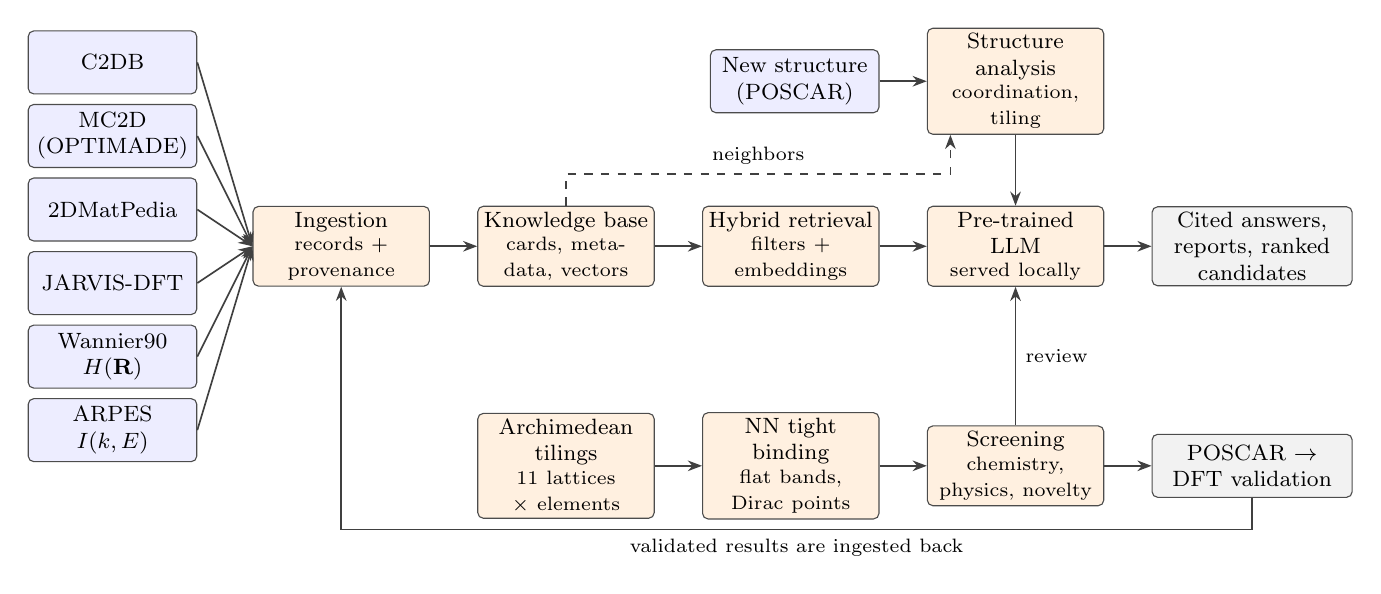
\begin{tikzpicture}[
  font=\footnotesize,
  box/.style={draw=black!70, rounded corners=2pt, align=center, minimum height=8mm,
              inner sep=2pt, text width=#1},
  box/.default=21mm,
  src/.style={box=20mm, fill=blue!7},
  stage/.style={box=21mm, fill=orange!12},
  outbox/.style={box=24mm, fill=black!5},
  arr/.style={-{Stealth[length=1.8mm]}, semithick, draw=black!75},
]
% data sources
\node[src] (c2db) {C2DB};
\node[src, below=1.2mm of c2db] (mc2d) {MC2D (OPTIMADE)};
\node[src, below=1.2mm of mc2d] (dmp) {2DMatPedia};
\node[src, below=1.2mm of dmp] (jar) {JARVIS-DFT};
\node[src, below=1.2mm of jar] (wan) {Wannier90 $H(\Rvec)$};
\node[src, below=1.2mm of wan] (arp) {ARPES $I(k,E)$};
\coordinate (mid) at ($(dmp.south east)!0.5!(jar.north east)$);
% retrieval-augmented pipeline
\node[stage, right=7mm of mid] (ing) {Ingestion\\[-1pt]\scriptsize records + provenance};
\node[stage, right=6mm of ing] (kb) {Knowledge base\\[-1pt]\scriptsize cards, metadata, vectors};
\node[stage, right=6mm of kb] (ret) {Hybrid retrieval\\[-1pt]\scriptsize filters + embeddings};
\node[stage, right=6mm of ret] (llm) {Pre-trained LLM\\[-1pt]\scriptsize served locally};
\node[outbox, right=6mm of llm] (ans) {Cited answers,\\ reports, ranked\\ candidates};
\foreach \s in {c2db,mc2d,dmp,jar,wan,arp} \draw[arr] (\s.east) -- (ing.west);
\draw[arr] (ing) -- (kb);
\draw[arr] (kb) -- (ret);
\draw[arr] (ret) -- (llm);
\draw[arr] (llm) -- (ans);
% analysis of a new structure
\node[stage, above=9mm of llm] (ana) {Structure analysis\\[-1pt]\scriptsize coordination, tiling};
\node[src, left=6mm of ana] (usr) {New structure (POSCAR)};
\draw[arr] (usr) -- (ana);
\draw[arr] (ana) -- (llm);
\draw[arr, dashed] (kb.north) -- ++(0,4mm) -| node[pos=0.25, above] {\scriptsize neighbors}
  ($(ana.south west)+(3mm,0)$);
% discovery loop
\node[stage, below=16mm of kb] (arch) {Archimedean tilings\\[-1pt]\scriptsize 11 lattices $\times$ elements};
\node[stage, right=6mm of arch] (tb) {NN tight binding\\[-1pt]\scriptsize flat bands, Dirac points};
\node[stage, right=6mm of tb] (scr) {Screening\\[-1pt]\scriptsize chemistry, physics, novelty};
\node[outbox, right=6mm of scr] (dft) {POSCAR $\rightarrow$\\ DFT validation};
\draw[arr] (arch) -- (tb);
\draw[arr] (tb) -- (scr);
\draw[arr] (scr) -- (dft);
\draw[arr] (scr) -- node[right] {\scriptsize review} (llm);
\draw[arr] (dft.south) -- ++(0,-4mm) -| node[pos=0.25, below] {\scriptsize validated results are ingested back}
  (ing.south);
\end{tikzpicture}
\caption{Architecture of LLMatter2D. Data sources are converted into records that keep
the method and provenance of every value; a hybrid retrieval layer supplies the relevant
records to a pre-trained language model served locally. New structures are analyzed against
the knowledge base, and the Archimedean generator proposes candidates that are screened,
reviewed by the model and exported for DFT; validated results re-enter the knowledge base.}
\label{fig:architecture}
\end{figure*}

\subsection{Data model and sources}

Each material is a record (Fig.~\ref{fig:architecture}) containing the slab geometry
(in-plane lattice vectors, vacuum vector and Cartesian sites), electronic properties (band
gaps, each labeled with its method, direct/indirect character, location in the Brillouin zone
and spin-orbit treatment; magnetic state and moment; Dirac cones, spin-orbit gaps and
topology; effective masses), stability (formation energy, energy above the convex hull,
exfoliation energy, dynamical stability, experimental realization), any number of
tight-binding models, any number of ARPES feature sets, free-text notes and a list of
provenance entries (source, identifier, method, reference, retrieval date). Records from
different sources keep source-prefixed identifiers (e.g., \code{mc2d:\ldots},
\code{c2db:\ldots}), which the language model is asked to cite.

Connectors are provided for MC2D through its OPTIMADE interface~\cite{Andersen2021}, for
local C2DB and 2DMatPedia files and for the JARVIS-DFT 2D dataset. The knowledge base used
in this work contains 3799 records: 2683 MC2D monolayers (1458 with a computed band gap),
1103 JARVIS-DFT monolayers (OptB88vdW gaps for all, TBmBJ gaps for 246 and HSE06 gaps for
54, together with formation and exfoliation energies, energies above the hull, magnetic
moments and average effective masses) and 13 curated records. A curated seed set of 13 well-known monolayers with literature values
(graphene, hBN, four $1H$ transition-metal dichalcogenides, $1T$-TaS$_2$, phosphorene,
silicene, germanene, stanene, CrI$_3$ and graphenylene)~\cite{CastroNeto2009,Mak2010,
Liu2011,Xu2013,Huang2017,Bostwick2007,Miwa2015,Zhang2014,Elias2019,Song2013} serves for
demonstrations and tests.

\subsection{Tight-binding and photoemission data}

Wannier90 Hamiltonians~\cite{Marzari2012,Pizzi2020} are read from \code{\_hr.dat} files,
dividing each matrix element by the degeneracy $N_{\Rvec}$ of its lattice vector,
\begin{equation}
  H_{mn}(\kvec) = \sum_{\Rvec} e^{2\pi i\,\kvec\cdot\Rvec}\,
  \frac{\tilde H_{mn}(\Rvec)}{N_{\Rvec}},
\end{equation}
with $\kvec$ in reduced coordinates; the largest hoppings are summarized in the text that
the model reads.

ARPES intensity maps $I(k,E)$ are reduced to quantities a language model can quote. The
dispersion of a band crossing the Fermi level is obtained from the maxima $k_m(E)$ of the
momentum distribution curves, refined below the grid spacing by a three-point parabola, and
the Fermi velocity follows from a linear fit, $v_F=\hbar^{-1}|dE/dk|$, within a window $w$
around $E_F$. Effective masses follow from a fit of the energy-distribution-curve maxima to
$E(k)=E_0+\hbar^2(k-k_0)^2/2m^*$. Each feature set stores the photon energy, temperature,
polarization and substrate of the measurement.

\subsection{Hybrid retrieval}

Every record is rendered as a short text card listing all values with their methods and
references, and as flat metadata (elements, range of band gaps over methods, magnetism,
Bravais lattice, tags, sources, availability of ARPES and tight-binding data). Numerical
or categorical constraints (e.g., a band gap between 1 and 2~eV, magnetic materials, records
with ARPES data) are applied as hard filters $\mathcal F$ on the metadata. The surviving
records are ranked by
\begin{equation}
  s_i = \hat{\mathbf q}\cdot\hat{\mathbf v}_i + \beta\,\delta_i, \qquad i\in\mathcal F,
\end{equation}
where $\hat{\mathbf q}$ and $\hat{\mathbf v}_i$ are normalized embeddings of the query and
of card $i$, and $\delta_i=1$ if the query contains the formula or the common name of the
material ($\beta=0.25$). Two embedders are available: a dependency-free feature-hashing
embedder~\cite{Weinberger2009} (2048 dimensions, words and character trigrams, with
chemical formulas kept case-sensitive), and dense sentence-transformer
models~\cite{Reimers2019}. For structure-based queries, known materials are ranked by
$S=\tfrac12 J+\tfrac12 e^{-\lVert\Delta\mathbf d\rVert}$, where $J$ is the Jaccard index of
the element sets and $\mathbf d=(a/5\,\text{\AA},\,b/5\,\text{\AA},\,\gamma/90^\circ,\,
N/6,\,h/3\,\text{\AA})$ collects the lattice parameters, the number of atoms per cell and the
layer thickness.

\subsection{Language models and prompts}

The default backend is a pre-trained instruction-tuned model served locally by
LM Studio~\cite{LMStudio} through its OpenAI-compatible endpoint (temperature 0.2;
reasoning blocks are removed from the answer); Ollama~\cite{Ollama} and hosted models are
also supported. The retrieved cards are wrapped in \code{<record id=\ldots>} blocks. The
system prompt instructs the model to treat the records as the source of numerical values,
to cite the record identifier after each value, to state the method behind every number and
recall that semilocal DFT underestimates band gaps, to separate computed, measured and
predicted values, and to say when the records do not contain the answer. Task-specific
prompts cover question answering, the analysis of a new structure and the review of
generated candidates.

\subsection{Archimedean tilings and tight binding}

The eleven Archimedean tilings are built as Bravais lattices with a basis of vertices and
unit edge length (Fig.~\ref{fig:tilings}); for instance, the snub square tiling
$3^2.4.3.4$ has a square cell of side $(2+\sqrt3)^{1/2}$ with four vertices, and the
truncated trihexagonal tiling $4.6.12$ has a hexagonal cell of side $\sqrt3(1+\sqrt3)$ with
twelve vertices. Bonds are all pairs at the minimum distance. The construction is checked
by the coordination number, by the equality of all bond lengths, and by the site density,
which must satisfy
\begin{equation}
  \rho^{-1} = \sum_{i=1}^{z}\frac{A(n_i)}{n_i}, \qquad A(n)=\frac{n}{4}\cot\frac{\pi}{n},
\end{equation}
for the vertex configuration $(n_1,\ldots,n_z)$; all eleven tilings satisfy it to
$10^{-9}$.

The nearest-neighbor model
\begin{equation}
  H_{ij}(\kvec) = -t\!\!\sum_{(i,j,\Rvec)\in\mathcal B}\!\! e^{i\kvec\cdot
  (\mathbf r_j+\Rvec-\mathbf r_i)} + \text{H.c.}
\end{equation}
is diagonalized on a $30\times30$ grid and along high-symmetry paths. A band is flat if its
width is below $10^{-6}t$. At each high-symmetry point, degenerate pairs are classified by the
ratio $r=\Delta E(2\delta)/\Delta E(\delta)$ of their splittings at distances $\delta$ and
$2\delta$ ($\delta=10^{-3}|\mathbf b_1|$), averaged over three directions: $r\approx2$
indicates a linear (Dirac-like) crossing and $r\approx4$ a quadratic touching; degeneracies
of more than two bands are reported separately.

Candidates are generated by placing one element on every vertex, or two elements on the
two sublattices of tilings that are bipartite within their primitive cell, with the bond
length estimated from covalent radii~\cite{Cordero2008}. Each candidate receives the score
$S=2C+E+N$, where $C$ is the mean over its elements of $+1$ ($-1$) if the coordination
number of the tiling is (is not) common for that element in covalent networks,
$E=\chi_{\text{flat}}+\chi_{\text{linear}}+\tfrac12\chi_{\text{quadratic}}$, with
$\chi=1$ if the tiling has the corresponding feature and $0$ otherwise,
and $N=\tfrac12$ unless the same element set on the same tiling is already present in the
knowledge base. The short list is reviewed by the language model with retrieved analogues and
exported as POSCAR files.

\subsection{Analysis of a new structure}

For a user-supplied slab, coordination numbers are computed with the criterion
$d_{AB}<1.2\,(r_A+r_B)$. The atoms are projected on the plane, coincident projections are
merged and the nearest-neighbor graph of the projected network is compared with the tilings
through its vertex degree and its scale-free density $\rho d^2$, which is independent of the
choice of supercell. These descriptors, the matched tilings with their tight-binding
features and the structurally closest known materials are passed to the model, which writes
an analysis report.

\subsection{Benchmark}

A benchmark question specifies the records $\mathcal R$ that contain the answer, and either
a reference value $q^\ast$ with unit and tolerance $\tau$ or keyword lists. For retrieval we
report recall@$k$, $|\mathcal R\cap\mathcal T_k|/|\mathcal R|$, where $\mathcal T_k$ are the
$k$ retrieved records, and the mean reciprocal rank (MRR). A numerical answer is correct if
it contains a quantity with the expected unit within $\tau$ of $q^\ast$; quantities are
parsed with conversion between eV and meV, \AA{} and nm, and m/s and km/s, including
scientific notation. For retrieval-augmented answers we also report the citation validity,
$|\mathcal C\cap\mathcal T_k|/|\mathcal C|$, and the citation precision,
$|\mathcal C\cap\mathcal R|/|\mathcal C|$, where $\mathcal C$ is the set of cited record
identifiers. Each question is asked to the same model with retrieval (RAG) and without it
(closed book).

Two question sets are used. The curated set contains 25 questions on the seed materials
(band gaps by method, spin-orbit gaps and splittings, Fermi velocity, hopping, lattice
constants, buckling, Curie temperature, magnetic order, charge-density waves, topology and
Archimedean structure). The database set contains 300 questions generated from the records
with a fixed random seed: 100 MC2D band gaps and 50 MC2D lattice constants, and 50
OptB88vdW gaps, 50 TBmBJ gaps and 50 lattice constants from JARVIS-DFT. Each question names
the database (e.g., ``What is the TBmBJ band gap of monolayer X in JARVIS-DFT?''), uses only
formulas that are unique within that database, skips metals (gaps below 0.1~eV) and, for
lattice constants, considers hexagonal and square cells only. Tolerances are
$\max(0.05~\text{eV}, 5\%)$ for gaps and $\max(0.03~\text{\AA}, 2\%)$ for lattice constants.
Because the reference value is the one stored in the database, a closed-book model can at
best approximate it, which is precisely the gap that retrieval is meant to close.

% =====================================================================================
\section{Results}
% =====================================================================================

\subsection{Electronic features of the Archimedean tilings}

\begin{figure*}[t]
\centering
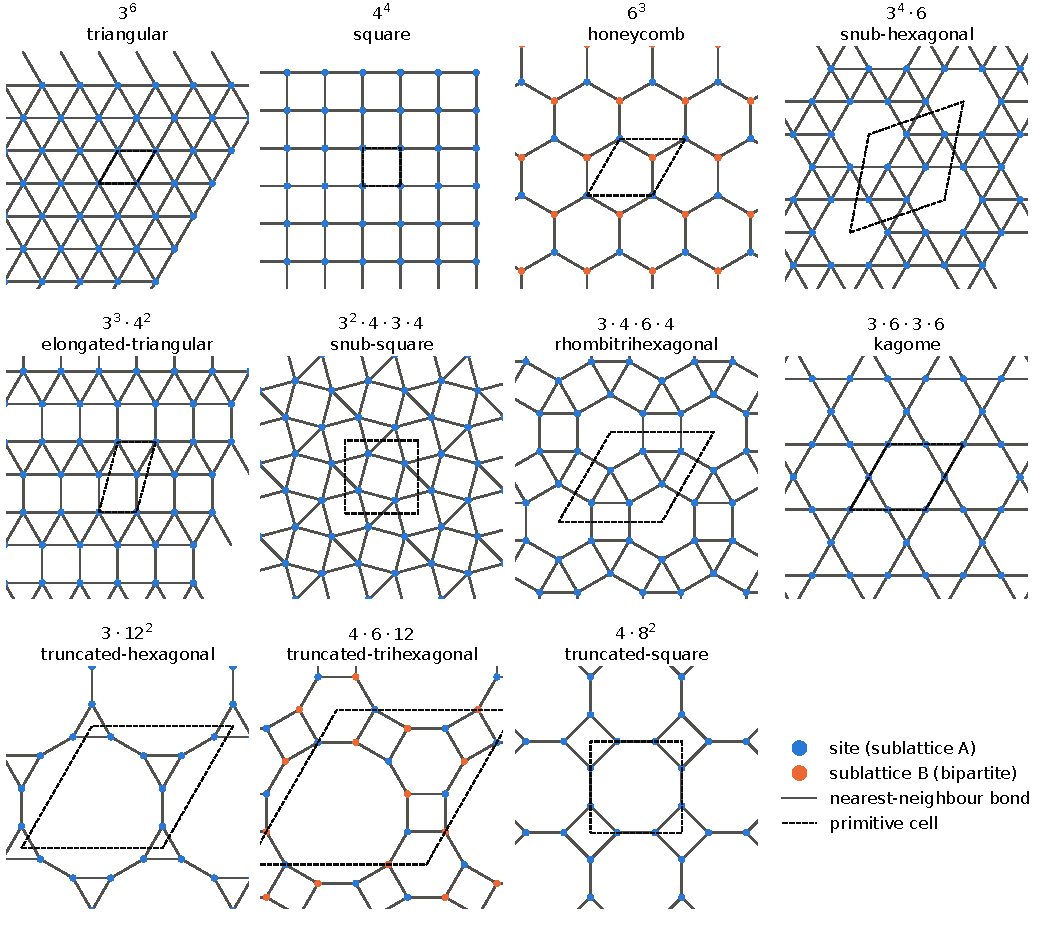
\includegraphics[width=0.92\textwidth]{archimedean_tilings}
\caption{The eleven Archimedean tilings generated by LLMatter2D, labeled by their vertex
configurations. Dashed lines show the primitive cells; orange sites mark the second
sublattice of the tilings that are bipartite within their primitive cell ($6^3$ and
$4.6.12$).}
\label{fig:tilings}
\end{figure*}

\begin{figure*}[t]
\centering
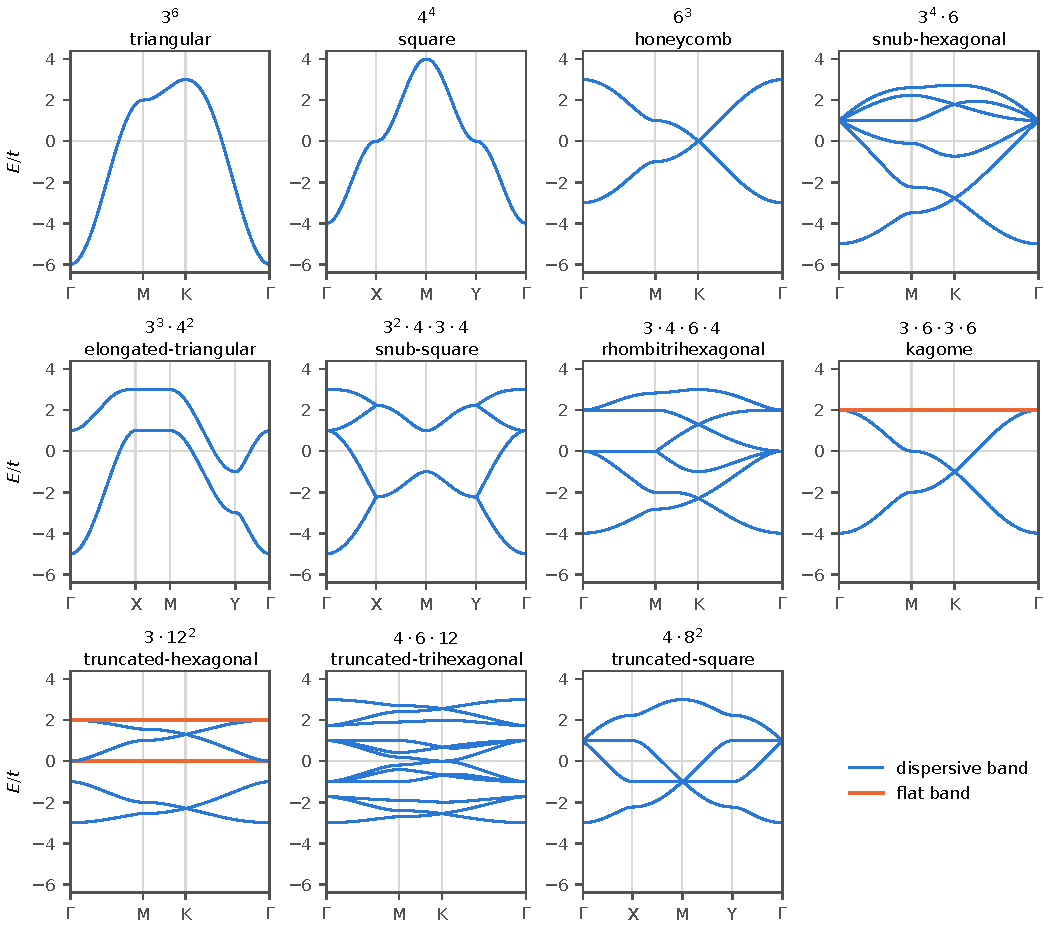
\includegraphics[width=0.92\textwidth]{archimedean_bands}
\caption{Nearest-neighbor tight-binding bands ($H=-t\sum_{\langle ij\rangle}c_i^\dagger
c_j+\text{H.c.}$) of the eleven tilings along high-symmetry paths. Flat bands are shown in
orange. For the oblique cell of $3^3.4^2$, X, M and Y denote $\mathbf b_1/2$,
$(\mathbf b_1+\mathbf b_2)/2$ and $\mathbf b_2/2$.}
\label{fig:bands}
\end{figure*}

\begin{table*}[t]
\caption{Geometry and nearest-neighbor band features of the Archimedean tilings: number of
sites $N$ per primitive cell, coordination $z$, site density $\rho$ in units of the bond
length $d$, bipartiteness within the primitive cell, energies of flat bands, and the
high-symmetry points hosting linear crossings, quadratic touchings and degeneracies of more
than two bands.}
\label{tab:tilings}
\footnotesize
\input{archimedean}
\end{table*}

Figures~\ref{fig:tilings} and~\ref{fig:bands} and Table~\ref{tab:tilings} summarize the
tilings. The honeycomb lattice shows the Dirac crossing at K and $E=0$ of
graphene~\cite{CastroNeto2009}. The kagome lattice $3.6.3.6$ has a flat band at $E=+2t$
that touches the dispersive bands quadratically at $\Gamma$, and a Dirac crossing at K at
$E=-t$~\cite{Sutherland1986}. The truncated hexagonal (star) lattice $3.12^2$ has two flat
bands, at $E=0$ and $E=+2t$, each with a quadratic touching at $\Gamma$, and Dirac crossings
at K at $E\simeq-2.303\,t$ and $1.303\,t$. The bipartite $4.6.12$ lattice has a spectrum
symmetric about $E=0$, with Dirac crossings at K at $E=\pm0.677\,t$ and $\pm2.558\,t$ and
threefold degeneracies at $\Gamma$ at $E=\pm t$. The snub square lattice $3^2.4.3.4$ has
linear crossings at X and Y at $E=\pm\sqrt5\,t$ and quadratic touchings at $\Gamma$ and M,
while $3^4.6$ shows a fivefold degeneracy at $\Gamma$ ($E=+t$) and $4.8^2$ threefold
degeneracies at $\Gamma$ ($+t$) and M ($-t$). These features are consistent with the Dirac
fermions, flat bands and high-degeneracy points reported for the Archimedean lattices in
Ref.~\onlinecite{CrastoDeLima2019}. The site densities of $3^3.4^2$ and $3^2.4.3.4$ coincide
($\rho d^2=1.072$) because both vertex configurations contain three triangles and two squares;
the structure matcher therefore returns both when only the degree and density are known.

The matcher identifies graphene, buckled silicene and the projected network of $1H$-MoS$_2$
as $6^3$, recovers $3.6.3.6$ for a decorated kagome layer and $4.8^2$ for a $2\times1$
supercell of the truncated square tiling.

\subsection{Extraction of photoemission observables}

On a synthetic map of an $n$-doped Dirac cone (Dirac point at $-0.4$~eV,
$v_F=10^6$~m/s, Lorentzian momentum width $0.01$~\AA$^{-1}$), the MDC analysis recovers
$v_F$ within $0.1\%$ using a $0.2$~eV window; on a noise-free parabolic band the fitted
effective mass agrees with the input ($m^\ast=0.5\,m_e$) to better than $10^{-6}$.
\pending{repeat with experimental data, e.g., graphene/SiC or epitaxial MoS$_2$, including noise
and finite resolution.}

\subsection{Candidate materials}

\begin{table}[t]
\caption{Highest-ranked new candidates for B, C, N, Si, Ge and Sn before any first-principles
calculation: tiling, coordination $z$, first-guess bond length $d$ from covalent radii,
flat bands, linear crossings and screening score.}
\label{tab:candidates}
\footnotesize
\input{candidates}
\end{table}

Decorating the eleven tilings with B, C, N, Si, Ge and Sn, and the two bipartite tilings
with all pairs of these elements, gives 96 candidates. The novelty check recovers graphene,
silicene, germanene, stanene and hBN on the $6^3$ tiling and graphenylene on $4.6.12$ as
known materials, which serve as benchmarks. Table~\ref{tab:candidates} lists the
highest-ranked new candidates. The kagome and star tilings dominate because they combine flat
bands with Dirac crossings, and many candidates share the same score: the screening is
coarse by design and only orders candidates for the more expensive steps. In particular, the
coordination prior ignores bond angles, so that, e.g., four-fold carbon with $60^\circ$ bond
angles on the kagome tiling is not penalized although it is chemically implausible; such
cases are exactly what the subsequent language-model review and DFT calculations must filter
out. \pending{DFT relaxation, phonon spectra, formation energies and energies above the hull
for the top candidates; band structures with spin-orbit coupling compared with the
tight-binding features; LLM review of the short list.}

\subsection{Retrieval}

\begin{table*}[t]
\caption{Retrieval on the 3799-record knowledge base: recall@$k$ (R@$k$) of the records that
hold the answer and mean reciprocal rank over the top 8, for the lexical (feature hashing) and
dense (BGE-small through sentence-transformers) embedders, with ($\beta=0.25$) and without
($\beta=0$) the bonus for exact formula or name matches.}
\label{tab:retrieval}
\footnotesize
\input{retrieval}
\end{table*}

Table~\ref{tab:retrieval} shows that the exact-match term is what makes retrieval reliable
for materials. Without it, the lexical embedder places the correct record first for only
25\% of the database questions (53\% within the top 8). Chemical formulas are split into
character trigrams shared by many compounds, and the remaining words of the question
(``band gap'', ``monolayer'', the database name) are common to thousands of cards. The dense
embedder is much better on its own (74\% at rank 1, 94\% within the top 8), but its errors are
chemically similar compounds, e.g., Cl$_9$K$_2$Ta$_3$ retrieved for Cl$_9$In$_2$Ta$_3$. With
the bonus, both embedders retrieve the correct record at rank 1 for 99.7--100\% of the 300
database questions. The curated questions expose a different difficulty: the same compound
is described by several records, and the answer (an optical gap, an ARPES splitting, a Curie
temperature) is only in the curated one. Here the lexical embedder with the bonus is best
(R@1 $=0.97$, R@3 $=1.00$) because the property words of the question appear in the right
card, whereas the dense embedder places the MC2D or JARVIS-DFT record of the same compound
first for MoS$_2$, MoSe$_2$ and CrI$_3$ (R@1 $=0.81$); the curated record still appears among
the eight records passed to the model (at ranks 2 to 6). Merging records of the same material across sources
would remove this ambiguity. The default configuration of LLMatter2D is therefore the lexical
embedder with the exact-match bonus, with dense embeddings as an option for free-text queries
that do not name a material.

\subsection{Answers of pre-trained models}

\pending{accuracy and citation metrics for RAG and closed-book answers on the 25 curated and
300 database questions, for at least three pre-trained models served by LM Studio, with model
identifiers, quantization, context length and repeated runs. Command:
\code{python paper/reproduce.py --llm lmstudio:<model>}.}

\subsection{Case study}

\pending{analysis of a monolayer absent from the knowledge base: descriptors, matched tiling,
closest known materials and the model's report, compared with a DFT calculation.}

% =====================================================================================
\section{Discussion}
% =====================================================================================

LLMatter2D separates what a language model is good at, namely reading, comparing and
explaining, from what it should not be trusted with, namely remembering numbers. All values
the model can quote come from records with a method and a reference, numerical constraints
are enforced outside the model, and electronic features of new lattices are computed rather
than guessed. Because the backend is a locally served pre-trained model, the full pipeline
runs without sending data to external services and different models can be compared on
identical context.

The present version has clear limitations. The tight-binding layer is restricted to one
orbital per site and nearest-neighbor hopping, without spin-orbit coupling; real materials
on these tilings will have additional orbitals, longer-range hoppings and distorted
geometries. The first-guess structures use covalent radii and must be relaxed. The screening
score is heuristic and ignores bond angles. The databases differ in functionals and
convergence settings, and records of the same material from different sources are not yet
merged automatically. The grading of numerical answers relies on pattern matching and the
keyword grading of textual answers is crude. Finally, answers of language models vary
between runs and models.

Natural extensions are Kane--Mele-type spin-orbit terms and $\mathbb Z_2$ invariants on the
Archimedean lattices~\cite{KaneMele2005,CrastoDeLima2019}, longer-range hoppings derived
from Wannier models~\cite{Liu2013TB}, ARPES data mined from the
literature~\cite{Shang2025}, pre-screening with machine-learned interatomic potentials and an
automated DFT loop that feeds validated candidates back into the knowledge base.

% =====================================================================================
\section{Conclusions}
% =====================================================================================

We have introduced LLMatter2D, a retrieval-augmented framework that grounds locally served
pre-trained language models in method-aware, citable data on two-dimensional materials and
couples them to a generator of new materials based on the Archimedean tilings.
\pending{main quantitative conclusions from the benchmark and from the DFT validation.}

\section*{Data availability}

The code, the benchmark questions, the scripts that generate every figure and table, and all
per-question outputs are available at \url{https://github.com/levsan13/LLMatter2D} under the
MIT license and archived on Zenodo~\cite{LLMatter2D}
(\href{https://doi.org/10.5281/zenodo.23779294}{doi:10.5281/zenodo.23779294}). The knowledge base was built on October 29,
2026 from the MC2D OPTIMADE endpoint (\url{https://optimade.materialscloud.org/main/mc2d},
2683 structures) and from the JARVIS-DFT 2D dataset distributed with \code{jarvis-tools}
(file \code{d2-12-12-2022.json.zip}, 1103 records; figshare DOI 10.6084/m9.figshare.6815705).
The 300 database questions, with their reference values and record identifiers, are part
of the repository, so the benchmark can be repeated even if the databases change.

\begin{acknowledgments}
\pending{funding and acknowledgments; disclosure of the use of AI-assisted tools in software
development and writing, following the journal policy.}
\end{acknowledgments}

\bibliography{references}

\end{document}
